\documentclass[conference]{IEEEtran}
\IEEEoverridecommandlockouts
% The preceding line is only needed to identify funding in the first footnote. If that is unneeded, please comment it out.
\usepackage{cite}
\usepackage{amsmath,amssymb,amsfonts}
\usepackage{algorithmic}
\usepackage{pdfpages}
\usepackage{graphicx}
\usepackage{textcomp}
\usepackage{xcolor}

\graphicspath{ {./} }
\pagestyle{plain}
\def\BibTeX{{\rm B\kern-.05em{\sc i\kern-.025em b}\kern-.08em
    T\kern-.1667em\lower.7ex\hbox{E}\kern-.125emX}}
    
\def\endthebibliography{%
  \def\@noitemerr{\@latex@warning{Empty `thebibliography' environment}}%
  \endlist
}
\makeatother
\begin{document}

\title{OpenDS: An Open Source Implementation of Discriminant Saliency on Center-surround Hypothesis\\
\thanks{A project proposal based on “On the plausibility of the discriminant center-surround hypothesis for visual saliency” by Dashan Gao; Vijay Mahadevan and Nuno Vasconcelos in 2008.}
}

\author{\IEEEauthorblockN{Yen Nhi Vuong}
\IEEEauthorblockA{\textit{EECS Department} \\
\textit{York University}\\
Toronto, Canada\\
ynhi97@my.yorku.ca}
}

\maketitle

\begin{abstract}
Most existing saliency detection models tend to target the high contrast in colors, intensity and orientation channels. However, it doesn’t accurately represent the visual focus of human. The saliency map most likely turns out to be a highlighted contour map of the image itself, rather than the actual focus point or region that people look at. In order to quantitatively predict human eye fixation on natural scenes, a research paper proposes saliency detection based on discriminant hypothesis. The discriminant saliency hypothesis is developed on top of the classical assumption that bottom-up saliency is a center-surround process. The methodology consists of two stages of detection, involving discriminant saliency detection, and leveraging natural image statistics to finally distinguish the target pop-out.
\end{abstract}

\begin{IEEEkeywords}
saliency, bottom-up, itti-koch, discriminant hypothesis, center-surround map
\end{IEEEkeywords}

\section{Introduction}
In computer vision, saliency is defined as standout part(s) of the image with distinct properties that draw eye fixation, which is the attention of the viewers. There are primary 2 saliency cues: \textit{bottom-up} - fast, stimulus-driven mechanism, and \textit{top-down} - slower, goal-driven mechanism \cite{Gao_Vasconcelos_2007}. Bottom-up saliency is more common in development as people tend to do it naturally without following certain tasks. Bottom-up is also highly desired because it allows us to understand what typically catches our attention, what visual features falls into the retina and so on...

The original research paper is called  \textit{"On the plausibility of the \textbf{discriminant center-surround hypothesis} for visual saliency”} by Dashan Gao \cite{Gao_Vasconcelos_2008}. \textbf{Discriminant analysis} concerns with classifying set of observed data into predefined classes, giving minimum probability of expected error. The analysis requires a discriminant function. The \textbf{center-surround} hypothesis suggests bottom-up saliency as a center-surround process that derives optimal saliency architecture. In this architecture, saliency is detected from discriminating between the centre area of interest (\textit{the center}) and the neighbourhood surrounding it (\textit{the surround}): The larger the difference between stimuli located at the centre and its surrounding is, the more salient the location becomes. Optimal saliency detectors can serve psychophysics predictions of human saliency such as eye fixation prediction on natural scenes, background subtraction on high dynamic scenes and motion-based saliency in the presence of ego-motion. 

The original research implemented a binary executable from MATLAB which is no longer working. This is an Engineering project which aims to reproduce the discriminant saliency model in Python 3 code with the help of open-source libraries such as OpenCV and Numpy.

\section{Methodology and Implementation}
The general architecture of image processing mainly follows the Itti-Koch-Niebur (IKN) model as shown in Figure \ref{fig:centersurround} \cite{Xu_2008}. Note that this is a slightly simpler and modified version compared to original Itti model, the differences will be discussed within this section.

On static imagery, the process consists of 2 main stages. First stage includes feature decomposition that results in intensity map \textit{I} and four color channels (\textit{R, G, B, and Y}). The feature maps are then convolved with three \textit{Mexican hat wavelet filters}. Mexican filters are centered at spatial frequencies 0.02, 0.04, and 0.08 cycles/pixel, to generate nine feature channels. Mexican hat wavelet is a linear difference filter for local area and feature point detection. In additional, the intensity map is convolved with (zero-mean) \textit{Gabor filter}. Gabor filter is a linear filter used for texture analysis; promotes the orientation/direction recognition. Gabor kernels filter at 3 spatial scales (centered at frequencies of 0.08, 0.16, and 0.32 cycles/pixel) and 4 directions (evenly spread from 0 to $\pi$). Due to challenges in implementation, the model was implemented with Gabor filter and some maths might not match up with research description. Mexican wavelet can be obtained through implemented function in Python package \texttt{PyWavelets - pywt}.

Next, in order to apply center-surround classification, the feature maps are worked into multi levels of Gaussian pyramid (implicitly called through OpenCV \texttt{pyrDown} function).
 
\begin{figure}[h]
    \centering
    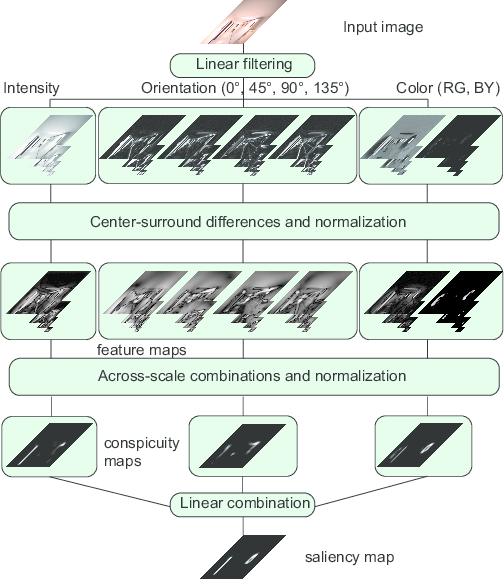
\includegraphics[width=3in]{itti.png}
    \caption{Itti-Koch model with center surround map computation}
    \label{fig:itti}
\end{figure}

The second stage aims to leverage image statistics by estimating the mutual information in Figure \ref{fig:mi_formula}. In short, the saliency of location $l$ is equated to the power of $\textbf{X}$ to discriminate between the center and surround of $l$ based on the distributions of the feature responses estimated from the two regions. However, this approach is deemed as impractical due to extensive computation on high-dimensional feature space. 

Alternative solution is represent such mutual information for high dimension through sum of marginal mutual information between every individual feature and its class labels, Figure \ref{fig:sum_formula}. Then each marginal mutual info is approximated by \textit{Generalized Gaussian distribution} (GGD). Gabor or wavelet (Laplace or Mexican wavelet) are band-pass filters such that mutual information can be estimated through the coefficients, which then reduces complexity of high dimensional image. Eventually it's possible to derive into new formula using Kullback–Leibler ($KL$) in Figure \ref{fig:kl_formula}.

\begin{figure}[h]
    \centering
    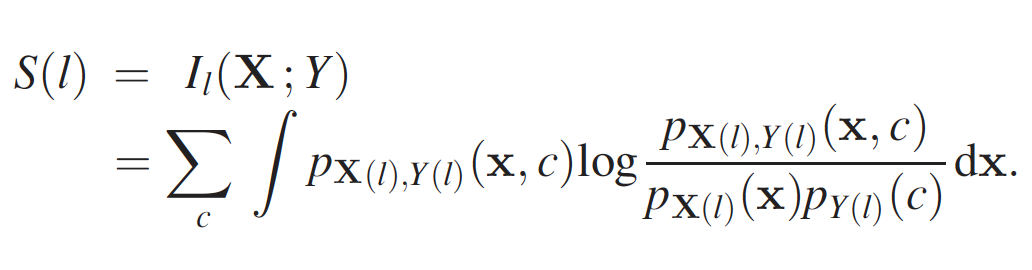
\includegraphics[width=2.5in]{MI.png}
    \caption{Formula for Saliency computation using Mutual Information (MI) Theory}
    \label{fig:mi_formula}
\end{figure}
  
\begin{figure}[h]
    \centering
    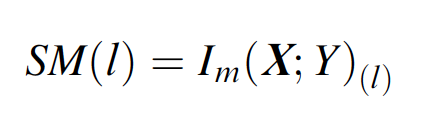
\includegraphics[width=1.5in]{alternative.png}
    \caption{Formula for Saliency computation as sum of marginal MIs}
    \label{fig:sum_formula}
\end{figure}
 
\begin{figure}[h]
    \centering
    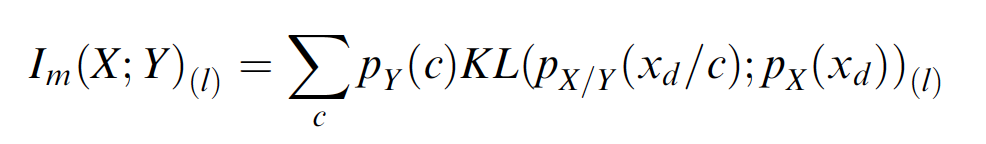
\includegraphics[width=2.5in]{KL.png}
    \caption{Formula for marginal MI computation using Kullback–Leibler divergence ($KL$) }
    \label{fig:kl_formula}
\end{figure}

\section{Test Data}
In order to test the model, image data was retrieved at the Toronto Dataset \cite{MITBenchmark_2012}. The images were collected under the research of Neil Bruce, John K. Tsotsos. \textit{Attention based on information maximization}. The dataset includes 120 color images of outdoor and indoor scenes. Each image is about size: 1024x768 pixels which helps minimize the processing time compared to an original photograph. The observers were 20 undergrads and grads student. The eye tracker device was ERICA workstation including a Hitachi CCD camera with an IR emitting LED.

In addition, large portion of images do not contain particular regions of interest which serve the purpose of testing the natural human fixation without any predictable features. 

Some other test images were collected directly from the research pdf. These images are not natural but rather synthetic data: solid, uniform background with consistent format objects (size, shape, color) on top. This data are more predictable.

\section{Results and Analysis}
The project final step would be to apply the implemented model to a set of input images, which is preferably close to the research’s original test set. Previously, the researchers relied on classical experiments in visual attention which were both qualitative and quantitative. For simple target pop-out test, some example images were provided directly in the research paper. And to generate human salience in natural indoors and outdoors, Toronto dataset is required.

\begin{figure}[h]
    \centering
    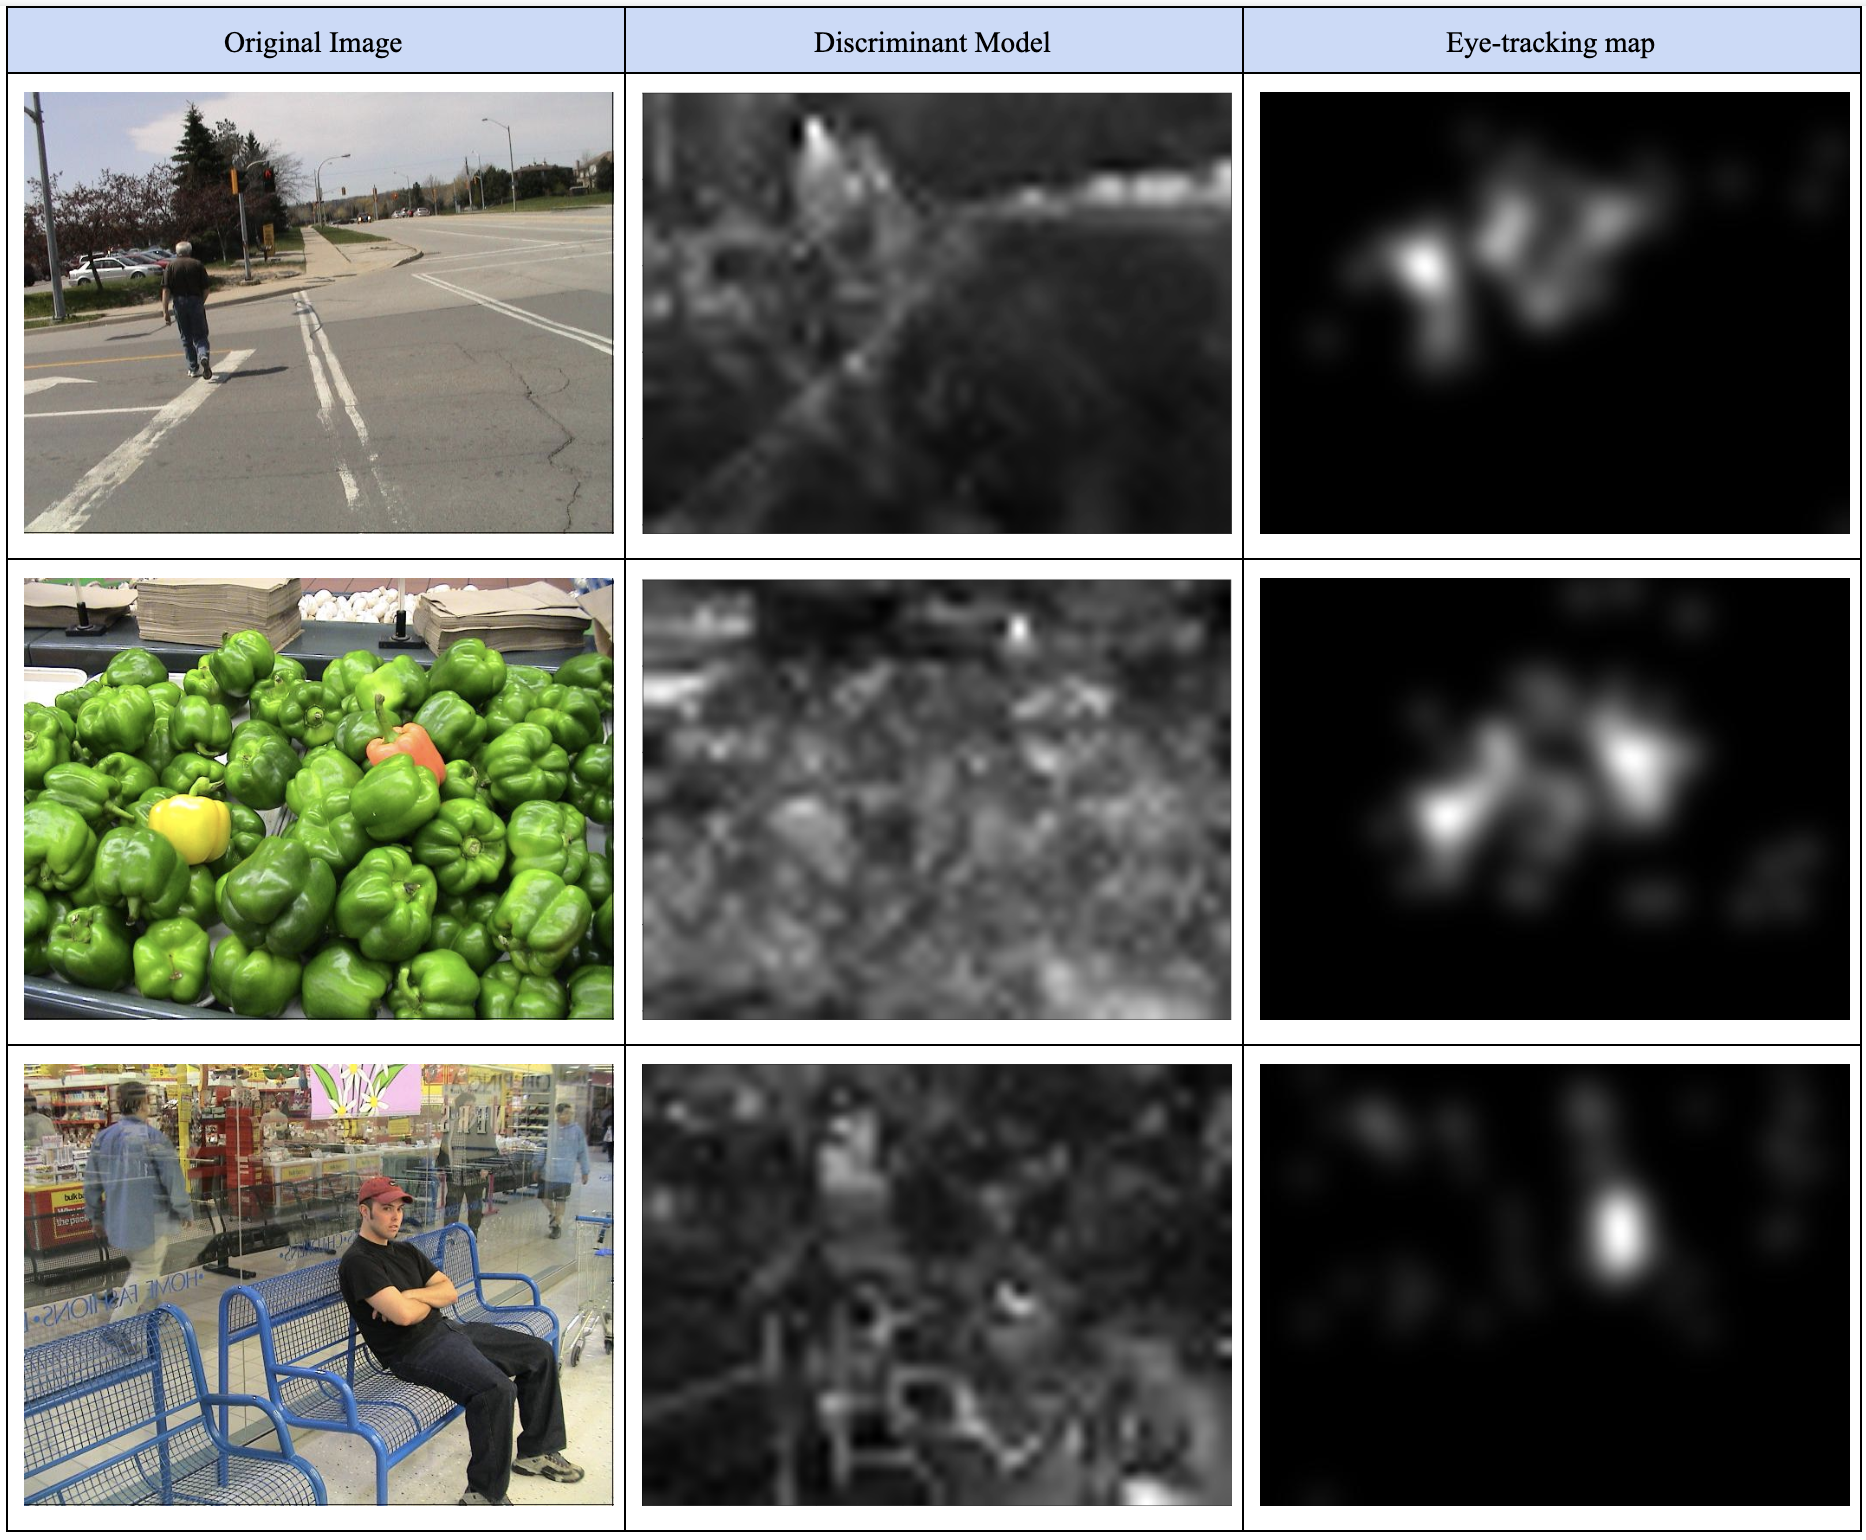
\includegraphics[width=3.5in]{outputs.png}
    \caption{Sample output table, from left to right: Original image, Discriminant map output and Actual eye-tracking data.) }
    \label{fig:outputs1}
\end{figure}

\begin{figure}[h]
    \centering
    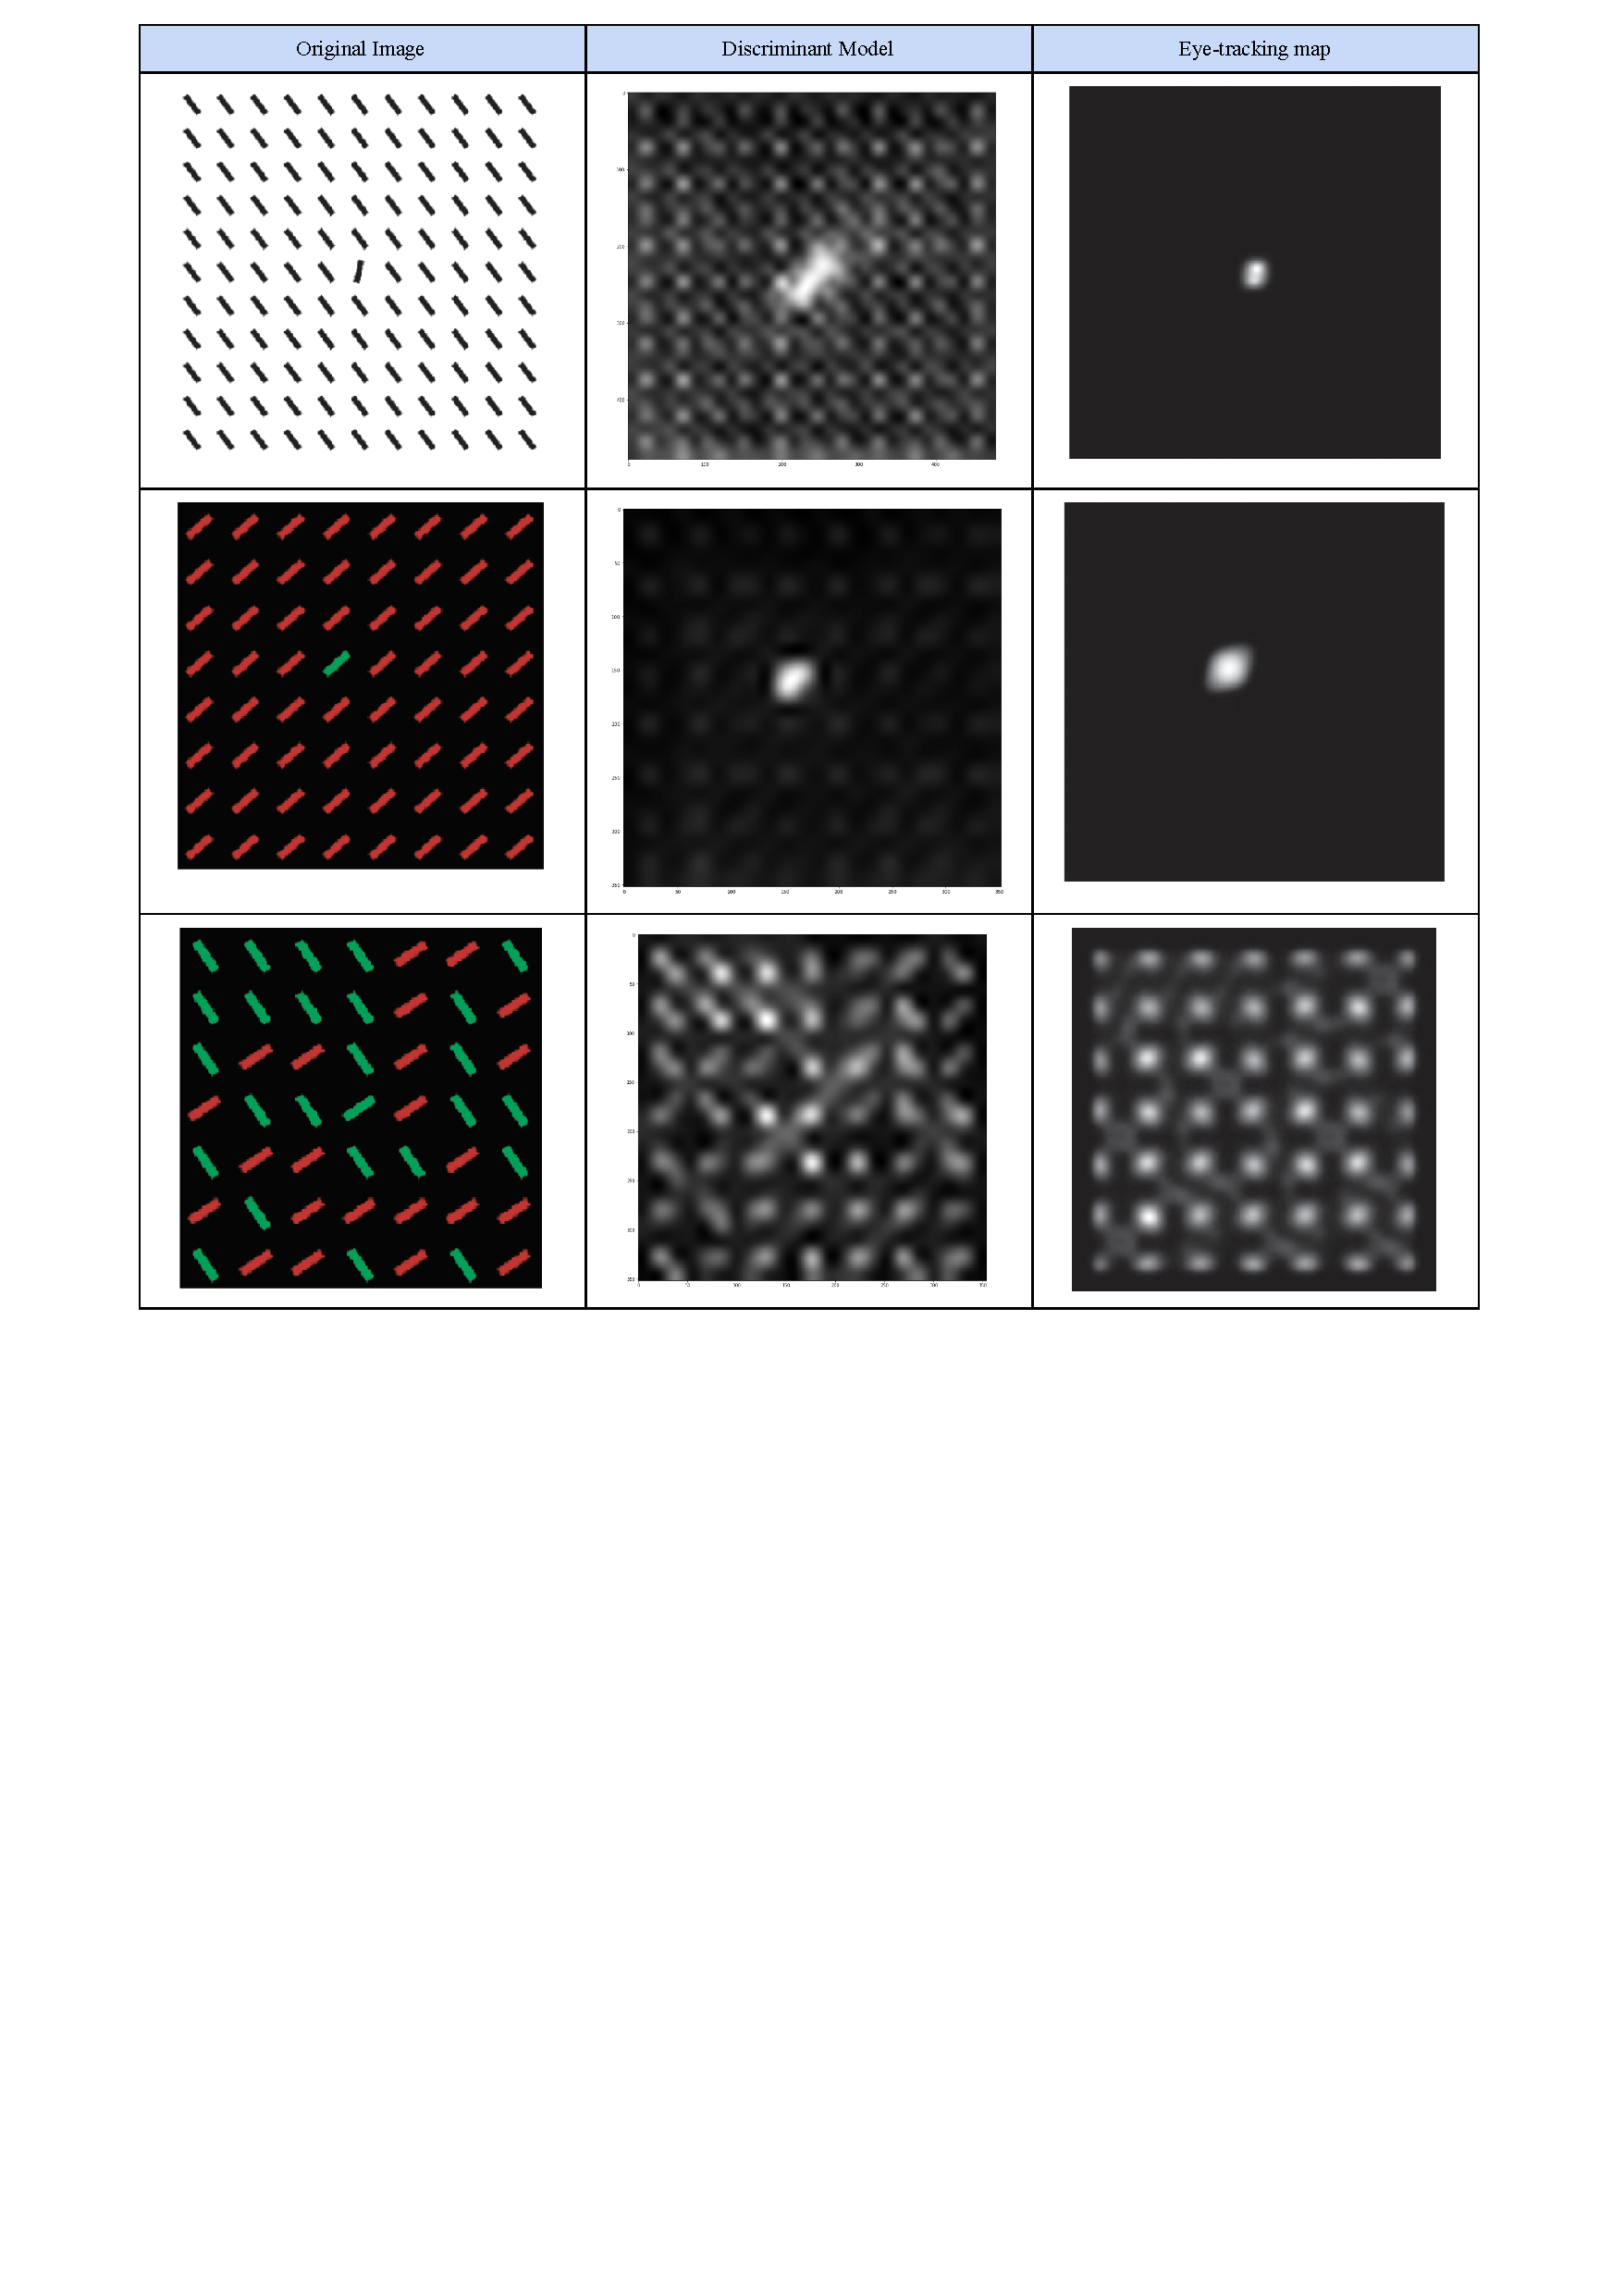
\includegraphics[trim={180 500 180 20},width=2.5in]{outputs2.pdf}
    \caption{Sample output table, from left to right: Original image, Discriminant map output and Actual eye-tracking data.) }
    \label{fig:outputs2}
\end{figure}

In Figure \ref{fig:outputs2}, Discriminant model was tested using synthetic data. The discriminant model made somewhat similar to ground-truth data (the eye-tracking map). The model performs relatively well in the situation of distinct orientation or color (the first two). Due to the fact that Gabor filter takes up majority of the implementation, the elongated diagonal bright lines can be seen in the third image. 

In Figure \ref{fig:outputs1}, the test images are from Toronto dataset. The generated saliency maps didn't perform as well. For example, in the first image, the model focus more on the distinct white paint with different orientation angle, rather than the human shape or tree. Then in the pepper example, there's a lot of details (as in line and contour) going on, and the model picks those up rather choosing the red, yellow peppers.

Therefore qualitative results of the discriminant implementation don't perform so well on actual indoor/outdoor scenery, but can detect simple synthetic image. 
\begin{figure}[h]
    \centering
    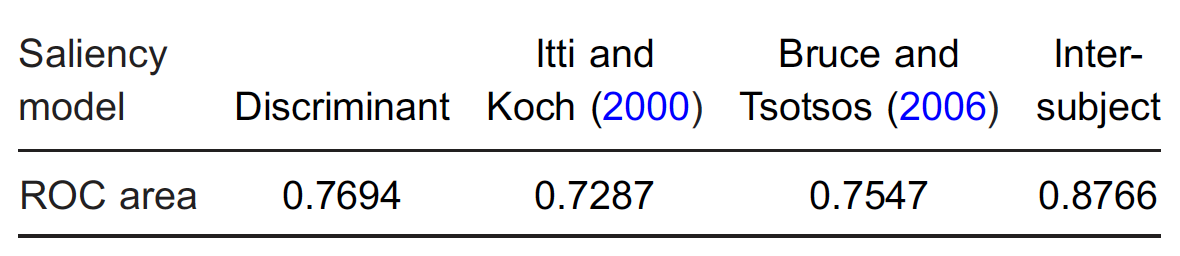
\includegraphics[width=2.5in]{score.png}
    \caption{ROC areas for different saliency models with respect to all human fixations.) }
    \label{fig:ROCscore}
\end{figure}


\begin{figure*}[h]
    \centering
    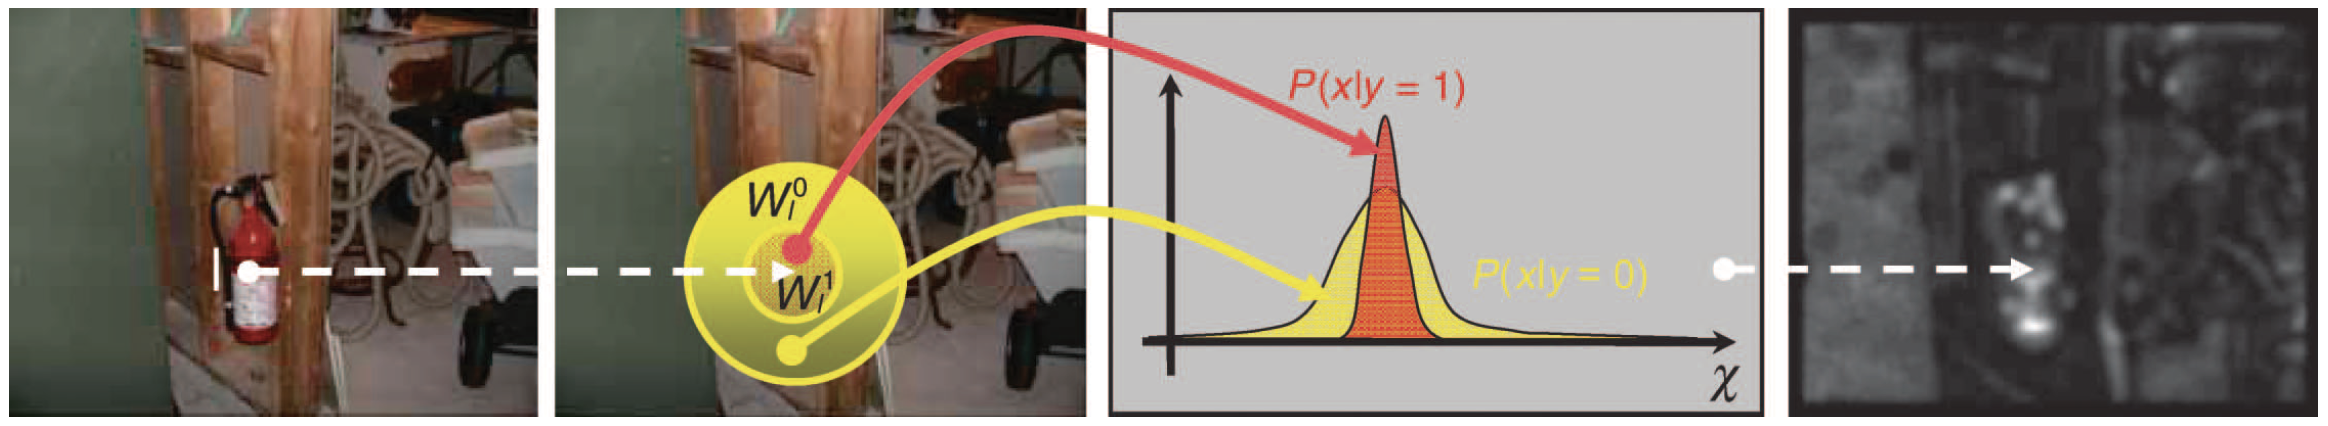
\includegraphics[width=6in]{research.png}
    \caption{ Illustration of discriminant center-surround saliency}
    \label{fig:centersurround}
\end{figure*}

\section{Code Repo}
OpenDS Github: \url{https://github.com/nhivuong/OpenDS}

\bibliographystyle{IEEEtran}
\bibliography{ref}

\end{document}
